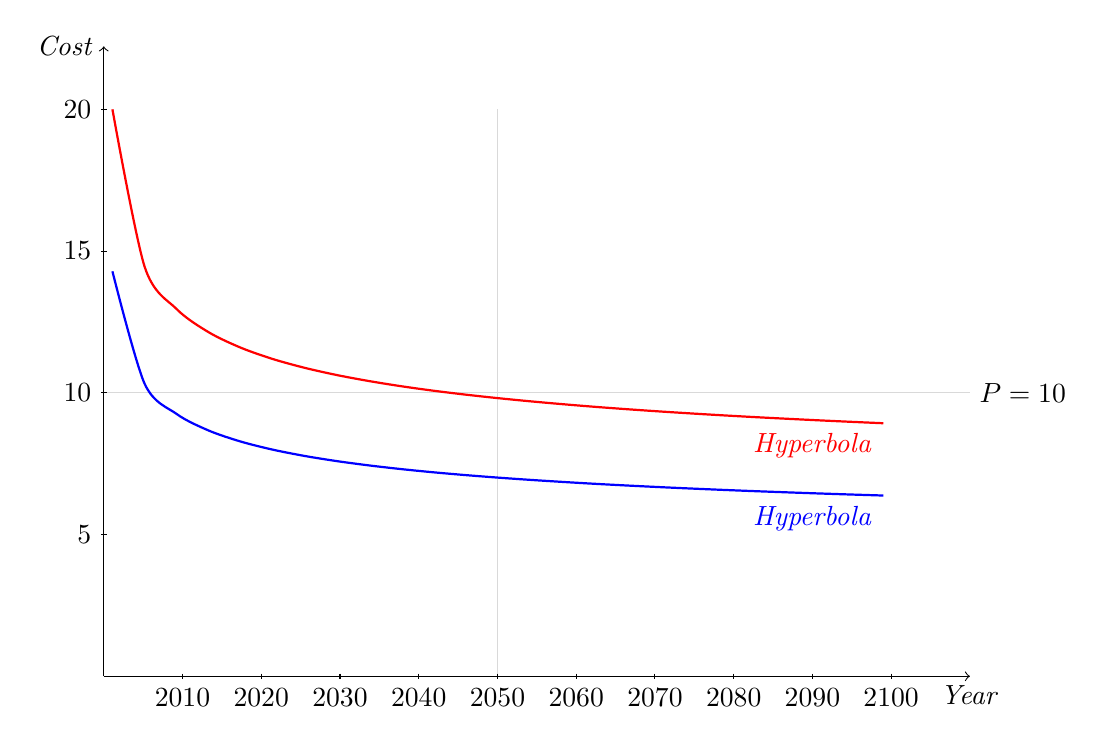
\begin{tikzpicture}
%\begin{tikzpicture}[x=1.2cm,y=0.4cm]

%\draw[help lines] (0,0) grid (13,13);

%  Draw the axes
\draw[->] (0,0) -- (11,0) node[below] {\emph{Year}};
\draw[->] (0,0) -- (0,8.0) node[left] {\emph{Cost}};

\draw[color=gray!30] (0,2*1.8) -- (11,2*1.8) node[right] {\color{black}{$P=10$}};
\draw[color=gray!30] (5,0) -- (5,4*1.8) node[below right] {};
%\draw[color=gray!30] (0,2) -- (2.5,2) node[below right] {\color{black}{$\eta=2.0$}} ;

\foreach \x in {1,...,10}
	\draw (\x cm, 1pt) -- (\x cm, -1pt) node[anchor = north]
	{\pgfmathparse{int(2000+10*\x)}${\pgfmathresult}$};

\foreach \y in {1,...,4}
	\draw (1pt, \y*1.8 cm) -- (-1pt, \y*1.8 cm) node[anchor = east]
	{\pgfmathparse{int(0+5*\y)}${\pgfmathresult}$};

\draw[scale=1,domain=0.11:9.9,smooth,variable=\x,red,thick] plot 
({\x},{(5+(20*(1-5/20))*((2110-2010)/11*\x)^(-ln((5/10-5/20)/(1-5/20))/ln(1/(2050-(2011-1)))))/(5/1.8)}) node[below left] {\emph{Hyperbola}};
\draw[scale=1,domain=0.11:9.9,smooth,variable=\x,blue,thick] plot 
({\x},{(5+(20*(1-5/20))*((2110-2010)/11*\x)^(-ln((5/10-5/20)/(1-5/20))/ln(1/(2050-(2011-1)))))/(7/1.8)}) node[below left] {\emph{Hyperbola}};
\end{tikzpicture}
